\pagestyle{empty}



\begin{frame}{Linear, affine, conic and convex hulls}  

Let   $X\subseteq\setR^n$: 
\begin{eqnarray*}
  \linhull(X) & = & \{ \lambda_1 x_1+ \cdots + \lambda_t x_t \mid t∈ ℕ_0,  \label{conv:eq:2}\\
   & & \quad \quad  x_1,\ldots,x_t
  \in  X, \, \lambda_1,\ldots,\lambda_t\in \setR\} \nonumber \\
  \affhull(X) & = & \{ \lambda_1 x_1+ \cdots + \lambda_t x_t \mid t ∈ ℕ_+, \label{conv:eq:4}\\
  & &   \quad \quad  x_1,\ldots,x_t \in  X, \, \sum_{i=1}^t \lambda_i = 1, \,
  \lambda_1,\ldots,\lambda_t\in \setR\} \nonumber   \\ 
  \cone(X)  & = & \{ \lambda_1 x_1+ \cdots + \lambda_t x_t \mid t∈ ℕ_0, \label{conv:eq:5} \\
  &&     \quad \quad  x_1,\ldots,x_t \in  X,  \, \lambda_1,\ldots,\lambda_t\in
  \setR_{\geq0}\} \nonumber \\
  \conv(X) & = & \{ \lambda_1 x_1+ \cdots + \lambda_t x_t \mid t ∈ ℕ_+, \label{conv:eq:6} \\
  &&     \quad \quad  x_1,\ldots,x_t \in  X, \,  \sum_{i=1}^t \lambda_i = 1, \, \lambda_1,\ldots,\lambda_t\in
  \setR_{\geq0}\} \nonumber 
\end{eqnarray*}

\end{frame}



\begin{frame}
  
\begin{figure}[htbp]
  \begin{center}
    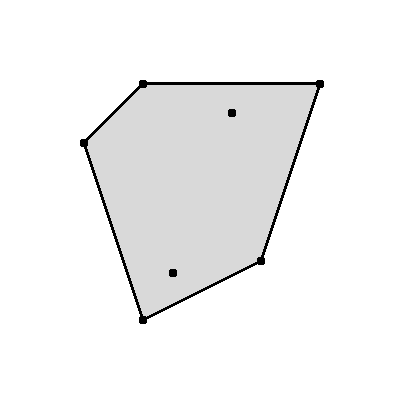
\includegraphics{../figures/picture1.pdf}    
  \end{center}
  \caption{The convex hull of $7$ points in $\setR^2$. }\label{conv:fig:2}
\end{figure}

\end{frame}


\begin{frame}
  
\begin{figure}[htbp]
  \begin{center}{
      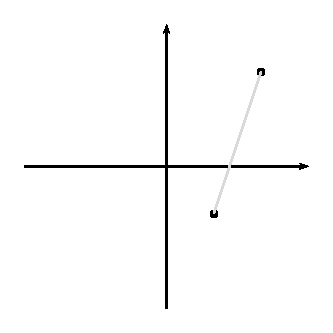
\includegraphics{../figures/picture2-1.pdf} 
      \hfill
      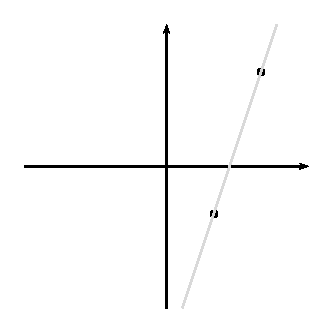
\includegraphics{../figures/picture2-2.pdf} 
    }
    
  \end{center}
  \caption{Two points with their convex hull on the left and  their
    affine hull on the right. }\label{conv:fig:1}
\end{figure}
\end{frame}



\begin{frame}
  

\begin{figure}[htbp]
  \begin{center}{
   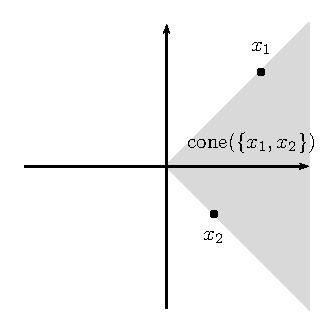
\includegraphics{../figures/picture3.pdf}

    }
    
  \end{center}
  \caption{Two points with their conic hull}\label{conv:fig:4}
\end{figure}

\end{frame}


\begin{frame}{Linear and affine hulls}


\begin{theorem}
  \label{conv:prop:1}
  Let $X\subseteq\setR^n$ and $x_0\in X$. One has 
  \begin{displaymath}
    \affhull(X) = x_0 + \linhull(X - x_0),
  \end{displaymath}
 
\end{theorem}

\bigskip
 where for $u \in \setR^n$ and $V\subseteq\setR^n$,   $u +V$ denotes the set
  $u+V = \{ u+v \mid v \in V\}$.
  
\end{frame}


\begin{frame}
  
\end{frame}

\begin{frame}
  
\end{frame}

\begin{frame}{Convex hull is convex}


\begin{theorem}
  \label{conv:thr:1}
  Let $X\subseteq\setR^n$ be a set of points. The convex hull, $\conv(X)$,  of $X$
  is convex. 
\end{theorem}

  
\end{frame}


\begin{frame}
  
\end{frame}

\begin{frame}{Convex hull is minimal}


\begin{theorem}
  \label{conv:thr:2}
  Let $X\subseteq\setR^n$ be a set of points. Each convex set $K$ containing $X$
  also contains $\conv(X)$. 
\end{theorem}
  
\end{frame}



\begin{frame}
  
\end{frame}


\begin{frame}{Corollary}


\begin{displaymath}
  \conv(X) = \bigcap_{\substack{K \supseteq X\\ K \text{  convex}}} K. 
\end{displaymath}
\end{frame}



\begin{frame}{Cones}
\begin{definition}
  \label{conv:def:4}
  A set $C\subseteq\setR^n$ is a \emph{cone}, if it is convex and for each $c \in
  C$ and each $\lambda \in \setR_{\geq0}$ one has  $\lambda\cdot c \in C$. 
\end{definition}
\end{frame}


\begin{frame}{Analogous theorems for cones} 
  \begin{theorem}
  \label{conv:thr:8}
  For any $X\subseteq\setR^n$, the set $\cone(X)$ is a cone. 
\end{theorem}

\begin{theorem}
  \label{conv:thr:9}
  Let $X\subseteq\setR^n$ be a set of points. Each cone containing $X$ also
  contains $\cone(X)$. 
\end{theorem}
\bigskip 
\begin{displaymath}
  \cone(X) = \bigcap_{\substack{C \supseteq X\\ C \text{  is a cone}}} C. 
\end{displaymath}
\end{frame}


\begin{frame}{Carathéodory's Theorem}

\begin{theorem}
  Let $X\subseteq\setR^n$, then for each $x \in \cone(X)$ there exists a set
  $\wt{X}\subseteq X$ of cardinality at most $n$  such that $x \in
  \cone(\wt{X})$. The vectors in $\wt{X}$ are linearly independent. 
\end{theorem}

\end{frame}



\begin{frame}
  
\end{frame}


\begin{frame}{Bounded continuous functions}

\begin{theorem}

  Let $X\subseteq\setR^n$ be compact and $f: X \to \setR$ be continuous. Then $f$ is
  bounded and there exist
  points $x_1,x_2 \in X$ with $f(x_1) = \sup\{ f(x) \colon  x \in X\}$ and
  $f(x_2) = \inf \{ f(x) \colon x \in X\}$. 
\end{theorem}
  
  \begin{columns}
    \begin{column}{.5\textwidth}
      
    \end{column}
    \begin{column}{.5\textwidth}
      
    \end{column}       
  \end{columns}
\end{frame}



\begin{frame}
  
\end{frame}

\begin{frame}{Separation theorem}

\begin{theorem}

  Let $K\subseteq\setR^n$ be a closed  convex set and $x^* \in \setR^n \setminus K$, then there
  exists an inequality $a^Tx ≤ \beta$ such that $a^T y < \beta$ holds for all
  $y \in K$ and $a^Tx^*>\beta$. 
\end{theorem}

  \begin{columns}
    \begin{column}{.5\textwidth}
      
    \end{column}
    \begin{column}{.5\textwidth}
      
    \end{column}       
  \end{columns}
\end{frame}






\begin{frame}{}

  \begin{columns}
    \begin{column}{.5\textwidth}
      
    \end{column}
    \begin{column}{.5\textwidth}
      
    \end{column}       
  \end{columns}
\end{frame}






\begin{frame}{Farkas' Lemma -- Version 1}



\begin{theorem}[Farkas' lemma]
  \label{conv:thr:12}
  Let $A \in \setR^{m\times n}$ be a matrix and $b \in \setR^m$ be a vector. The
  system $Ax = b, \,x\geq0$ has a solution if and only if for all $\lambda \in
  \setR^m$ with $\lambda^TA\geq0$ one has $\lambda^Tb \geq0$.  
\end{theorem}
  
  \begin{columns}
    \begin{column}{.5\textwidth}
      
    \end{column}
    \begin{column}{.5\textwidth}
      
    \end{column}       
  \end{columns}
\end{frame}





\begin{frame}{}

  \begin{columns}
    \begin{column}{.5\textwidth}
      
    \end{column}
    \begin{column}{.5\textwidth}
       
    \end{column}       
  \end{columns}
\end{frame}






\begin{frame}{Farkas' Lemma -- Version 2}

\begin{theorem}[Farkas' lemma]
  \label{conv:thr:12}
  Let $A \in \setR^{m\times n}$ be a matrix and $b \in \setR^m$ be a vector. The
  system $Ax ≤ b$ has a solution if and only if for all $\lambda \in
  \setR_{≥0}^m$ with $\lambda^TA = 0$ one has $\lambda^Tb \geq0$.  
\end{theorem}

\bigskip 
Exercise! 
 
\end{frame}





%%% Local Variables:
%%% mode: LaTeX
%%% TeX-master: "Slides"
%%% End:
